\documentclass[letterpaper]{article} % DO NOT CHANGE THIS
\usepackage[submission]{aaai25}  % DO NOT CHANGE THIS
\usepackage{times}  % DO NOT CHANGE THIS
\usepackage{helvet}  % DO NOT CHANGE THIS
\usepackage{courier}  % DO NOT CHANGE THIS
\usepackage[hyphens]{url}  % DO NOT CHANGE THIS
\usepackage{graphicx} % DO NOT CHANGE THIS
\urlstyle{rm} % DO NOT CHANGE THIS
\def\UrlFont{\rm}  % DO NOT CHANGE THIS
\usepackage{natbib}  % DO NOT CHANGE THIS AND DO NOT ADD ANY OPTIONS TO IT
\usepackage{caption} % DO NOT CHANGE THIS AND DO NOT ADD ANY OPTIONS TO IT
\frenchspacing  % DO NOT CHANGE THIS
\setlength{\pdfpagewidth}{8.5in} % DO NOT CHANGE THIS
\setlength{\pdfpageheight}{11in} % DO NOT CHANGE THIS

\usepackage[linesnumbered,ruled,vlined]{algorithm2e}
\usepackage{microtype}
\usepackage{mathtools}
\usepackage{forest}
\usepackage{siunitx}
\usepackage{amsfonts}
\usepackage{pifont}
\usepackage[inline]{enumitem}
\usepackage[capitalize,noabbrev]{cleveref}
\usepackage{booktabs}
\usepackage{amsthm}

\newtheorem{theorem}{Theorem}
\newtheorem{assumption}{Assumption}
\newtheorem{corollary}{Corollary}
\newtheorem{fact}{Observation}
\newtheorem{lemma}{Lemma}
\theoremstyle{remark}
\newtheorem*{remark}{Remark}
\theoremstyle{definition}
\newtheorem{definition}{Definition}
\newtheorem{example}{Example}

\usetikzlibrary{arrows.meta}
\usetikzlibrary{positioning}

\forestset{
  sn edges/.style={for tree={edge={-Latex}}}
}

\newcommand{\cmark}{\ding{51}}
\newcommand{\xmark}{\ding{55}}
\newcommand{\expr}{\mathtt{expr}}
\newcommand{\Ctwo}{$\mathsf{C}^{2}$}
\newcommand{\FO}{$\mathsf{FO}$}
\newcommand{\UFO}{$\mathsf{UFO}^{2} + \mathsf{CC}$}
\newcommand{\Cranetwo}{\textsc{Crane2}}
\newcommand{\Cranebfs}{\textsc{Crane2-BFS}}
\newcommand{\Cranegreedy}{\textsc{Crane2-Greedy}}

\newcommand{\crefrangeconjunction}{--}
\crefname{line}{line}{lines}
\crefname{fact}{Observation}{Observations}
\crefname{assumption}{Assumption}{Assumptions}
\crefalias{enumi}{type}
\crefname{type}{Type}{Types}
\creflabelformat{type}{#2\textup{#1}#3}
\crefalias{enumi}{step}
\crefname{step}{Step}{Steps}
\creflabelformat{step}{#2\textup{#1}#3}
\crefalias{clause}{equation}
\crefname{clause}{Clause}{Clauses}
\creflabelformat{clause}{#2\textup{(#1)}#3}
\crefalias{formula}{equation}
\crefname{formula}{Formula}{Formulas}
\creflabelformat{formula}{#2\textup{(#1)}#3}

\DeclareMathOperator{\CR}{CR}
\DeclareMathOperator{\DR}{DR}
\DeclareMathOperator{\Reff}{Ref}
\DeclareMathOperator{\Doms}{Doms}

\SetKwFunction{CompileWithBaseCases}{CompileWithBaseCases}
\SetKwFunction{Compile}{{\normalfont \textsc{Crane}}}
\SetKwFunction{Propagate}{Propagate}
\SetKwFunction{FindBaseCases}{FindBaseCases}
\SetKwFunction{Simplify}{Simplify}

\pdfinfo{
/TemplateVersion (2025.1)
}

\setcounter{secnumdepth}{2} %May be changed to 1 or 2 if section numbers are desired.

\title{Towards Practical First-Order Model Counting}
\author{Anonymous Submission}
\affiliations{}

\begin{document}

\maketitle

\begin{abstract}
  First-order model counting (FOMC) is the problem of counting the number of
  models of a sentence in first-order logic. Recently, a new algorithm for FOMC
  was proposed that, instead of simply providing the final count, generates
  definitions of (possibly recursive) functions, which can be evaluated with
  different arguments to compute the model count for any domain size. However,
  the algorithm did not include base cases in the recursive definitions. This
  work makes three contributions. First, we demonstrate how to construct
  function definitions that include base cases by modifying the logical formulas
  used in the FOMC algorithm. Second, we extend the well-known circuit
  modification technique in knowledge compilation, known as smoothing, to work
  with the formulas corresponding to base cases. Third, we introduce a
  compilation algorithm that transforms the function definitions into C++ code,
  equipped with arbitrary-precision arithmetic. These additions allow the new
  FOMC algorithm to scale to domain sizes over \num{500000} times larger than
  the current state of the art, as demonstrated through experimental results.
\end{abstract}

% TODO: Having an algorithm that can efficiently handle large domain sizes is
% crucial in the weighted setting. For example, consider the well-known "friends
% and smokers" Markov logic network [1]. The utility of such a model would be
% significantly limited if exact probabilities could only be efficiently
% computed for social networks of at most 30 people.
% [1] Richardson, M., & Domingos, P. (2006). Markov logic networks. Machine learning, 62, 107-136.

% TODO: (somewhere) The implementation is only for unweighted (but the
% definition of WFOMC is still necessary because of Skolemization).

% TODO: consider restructuring the paper (how?)

\section{Introduction}
% TODO: make it extra clear what the gap is that this work is trying to fill

% TODO: mention Crane earlier and describe its importance

% TODO: the last two paragraphs should make more of a BOOM (e.g., include the
% over 9k claim)

% TODO (here and elsewhere): clarify the distinction between the weighted and
% unweighted variants of the problem in the final version of the paper. We focus
% on the unweighted variant in our implementation and experiments, however,
% Crane2 can handle WFOMC instances as well simply by switching the main data
% type from integers to rational numbers. Maybe add some weighted experiments as
% well.

% TODO: (must) more related work, situating my contributions in the broader
% context

% TODO: (concerning related work) the topic is intimately related to "graded
% logics", largely investigated in DL, mu-calculus and temporal logics

% 1. What is the problem?

\emph{First-order model counting} is the task of counting the number of models
of a sentence in first-order logic over some given domain(s). The (symmetric)
weighted variant of this problem, known as WFOMC, seeks to calculate the sum of
model weights. In WFOMC, the weight of a model is determined by predicate
weights~\cite{DBLP:conf/ijcai/BroeckTMDR11}. WFOMC is a key approach to
\emph{lifted (probabilistic) inference}, which aims to compute probabilities
more efficiently by leveraging symmetries inherent in the problem
description~\cite{DBLP:conf/ecai/Kersting12}.

% 2. Why is it interesting and important?

Lifted inference is an active area of research, with recent work in domains such
as constraint satisfaction problems~\cite{DBLP:journals/jair/TotisDRK23} and
probabilistic answer set programming~\cite{DBLP:journals/ijar/AzzoliniR23}.
WFOMC has been used for inference on probabilistic
databases~\cite{DBLP:journals/debu/GribkoffSB14} and probabilistic logic
programs~\cite{DBLP:journals/ijar/RiguzziBZCL17}. By considering domains of
increasing sizes, the model count of a formula can be seen as an integer
sequence. WFOMC algorithms have been utilised for discovering new
sequences~\cite{DBLP:conf/ijcai/SvatosJT0K23} as well as
conjecturing~\cite{DBLP:conf/ilp/BarvinekB0ZK21} and
constructing~\cite{DBLP:conf/kr/DilkasB23} recurrence relations and other
recursive structures that describe these sequences. Additionally, WFOMC
algorithms have been extended to perform
\emph{sampling}~\cite{DBLP:conf/aaai/WangB0K22,DBLP:conf/lics/WangP0K23}.

% 3. Why is it hard? (E.g., why do naive approaches fail?)

The complexity of WFOMC is typically characterised in terms of \emph{data
  complexity}. This involves fixing the formula and determining whether an
algorithm exists that can compute the WFOMC in time polynomial with respect to
the domain size(s). If such an algorithm exists, the formula is called
\emph{liftable}~\cite{DBLP:conf/starai/JaegerB12}.
\citeauthor{DBLP:conf/pods/BeameBGS15}~\shortcite{DBLP:conf/pods/BeameBGS15}
demonstrated the existence of an unliftable formula with three variables. It is
also known that all formulas with up to two variables are
liftable~\cite{DBLP:conf/nips/Broeck11,DBLP:conf/kr/BroeckMD14}. The liftable
fragment of formulas with two variables has been expanded with various
axioms~\cite{DBLP:conf/aaai/TothK23,DBLP:journals/ai/BremenK23}, counting
quantifiers~\cite{DBLP:journals/jair/Kuzelka21} and in other
ways~\cite{DBLP:conf/nips/KazemiKBP16}.

% 4. Why hasn't it been solved before? (Or, what's wrong with previous proposed
% solutions? How does mine differ?)

There are various WFOMC algorithms with different underlying principles. Perhaps
the most prominent class of WFOMC algorithms is based on \emph{first-order
  knowledge compilation} (FOKC). In this approach, the formula is compiled into
a representation (such as a circuit or graph) by iteratively applying
\emph{compilation rules}. This representation can then be used to compute the
WFOMC for any combination of domain sizes (or weights). Algorithms in this class
include \textsc{ForcLift}~\cite{DBLP:conf/ijcai/BroeckTMDR11} and its recent
extension \textsc{Crane}~\cite{DBLP:conf/kr/DilkasB23}. The former compiles
formulas into circuits, while the latter compiles them first to graphs and then
to (algebraic) equations. Another WFOMC algorithm,
\textsc{FastWFOMC}~\cite{DBLP:conf/uai/BremenK21}, is based on cell enumeration.
Other algorithms utilise local search~\cite{DBLP:journals/pvldb/NiuRDS11},
junction trees~\cite{DBLP:conf/aaai/VenugopalSG15}, Monte Carlo
sampling~\cite{DBLP:journals/cacm/GogateD16}, and anytime approximation via
upper/lower bound construction~\cite{DBLP:conf/ijcai/BremenK20}.

% 5. What are the key components of my approach and results? Also include any
% specific limitations.

% TODO: introduce MLNs somewhere? maybe use an acronym?
The recently proposed \textsc{Crane} algorithm, while capable of handling
formulas beyond the reach of \textsc{ForcLift}, was `incomplete' as it could
only construct function definitions, which would then need to be evaluated to
compute the WFOMC.\@ In other words, it could not be used as a black box that
takes Markov logic networks (or weighted formulas in some other format) and
outputs numbers (i.e., model counts or probabilities). Additionally, recursive
functions were presented without base cases. In this work, we introduce
\Cranetwo{}, an extension of \textsc{Crane} that addresses these two weaknesses.

\begin{figure*}[t]
  \centering
  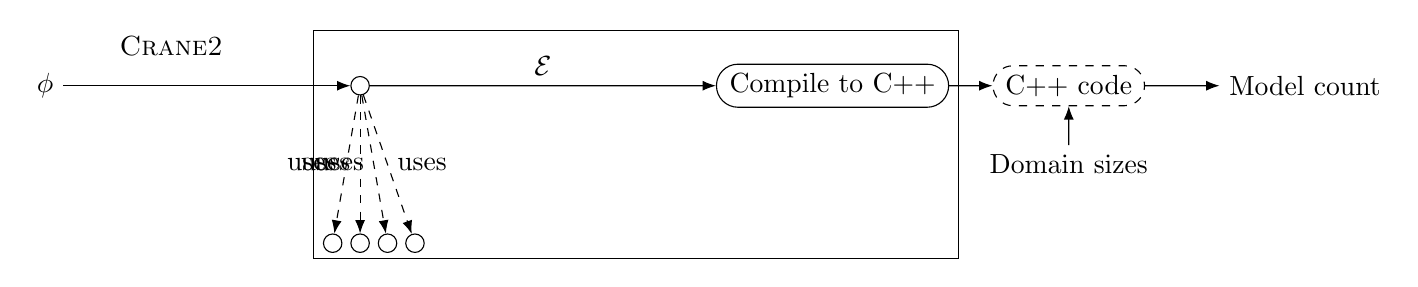
\begin{tikzpicture}
    \node at (-1, 0) (formula) {$\phi$};
    \node[draw,rounded rectangle] at (3, 0) (compilewithbasecases) {\CompileWithBaseCases};
    \node[draw,rounded rectangle] at (9, 0) (compilation) {Compile to C++};

    \node[draw,rounded rectangle,dashed] at (12, 0) (cpp) {C++ code};
    \node at (12, -1) (sizes) {Domain sizes};

    \node at (15, 0) (count) {Model count};

    \node[draw,rounded rectangle] at (3, -2) (findbasecases) {\FindBaseCases};
    \node[draw,rounded rectangle,left = 0.1cm of findbasecases] (crane) {\Compile};
    \node[draw,rounded rectangle,right = 0.1cm of findbasecases] (propagate) {\Propagate};
    \node[draw,rounded rectangle,right = 0.1cm of propagate] (simplify) {\Simplify};

    \node[draw,fit={(compilewithbasecases) (compilation) (crane) (findbasecases) (propagate)},inner ysep=7pt,yshift=5pt] {};
    \node at (0.6, 0.5) {\Cranetwo};

    \draw[-Latex] (formula) -- (compilewithbasecases);
    \draw[-Latex] (compilewithbasecases) -- node[above] {$\mathcal{E}$} (compilation);
    \draw[-Latex] (compilation) -- (cpp);
    \draw[-Latex] (sizes) -- (cpp);
    \draw[-Latex] (cpp) -- (count);

    \draw[-Latex,dashed] (compilewithbasecases) -- node[midway,left] {uses} (crane);
    \draw[-Latex,dashed] (compilewithbasecases) -- node[midway,left] {uses} (findbasecases);
    \draw[-Latex,dashed] (compilewithbasecases) -- node[midway,left] {uses} (propagate);
    \draw[-Latex,dashed] (compilewithbasecases) -- node[midway,right] {uses} (simplify);
  \end{tikzpicture}
  \caption[]{The outline of using \Cranetwo{} to compute the model count of a formula $\phi$. First, the formula is compiled into a set of equations, which are then used to create a C++ program. This program can be executed with different command line arguments to calculate the model count of $\phi$ for different domain sizes. To accomplish this, the \CompileWithBaseCases function employs several components:
    \begin{enumerate*}[label=(\roman*)]
      \item the FOKC algorithm of \textsc{Crane},
      \item a procedure called \FindBaseCases, which identifies a sufficient set of base cases,
      \item a procedure called \Propagate, which constructs a formula corresponding to a given base case, and
      \item algebraic simplification techniques (denoted as \Simplify).
    \end{enumerate*}
  }\label{fig:overview}
\end{figure*}

\Cref{fig:overview} outlines the workflow of the new algorithm. In
\cref{sec:main}, we describe how \CompileWithBaseCases finds the base cases for
recursive functions by:
\begin{enumerate*}[label=(\roman*)]
  \item identifying a sufficient set of base cases for each function,
  \item constructing formulas corresponding to these base cases,
  and\label[step]{step2}
  \item recursing on these new formulas.
\end{enumerate*}
Then, \cref{sec:smoothing} explains post-processing techniques for the formulas
from \cref{step2} above required to preserve the correct model count. Next,
\cref{sec:cpp} elucidates how function definitions encoding a solution to a
WFOMC problem are compiled into C++ programs. Note that a solution to WFOMC that
uses compilation to C++ has been considered
before~\cite{DBLP:conf/kr/KazemiP16}, however, the extent of formulas that could
be handled was limited. Finally, \cref{sec:experiments} presents experiments
results comparing \Cranetwo{} with other state-of-the-art WFOMC algorithms.

\section{Preliminaries}

In \cref{sec:logic}, we provide a summary of the basic principles of first-order
logic. Then, in \cref{sec:threelogics}, we formally define WFOMC and discuss the
distinctions between three variations of first-order logic that are utilised for
WFOMC.\@ Finally, in \cref{sec:algebra}, we introduce the terminology used to
describe the output of the original \textsc{Crane} algorithm, i.e., functions
and equations that define them.

We use $\mathbb{N}_{0}$ to represent the set of non-negative integers. In both
algebra and logic, we write $S\sigma$ to denote the application of a
\emph{substitution} $\sigma$ to an expression $S$, where
$\sigma = [x_{1} \mapsto y_{1}, x_{2} \mapsto y_{2}, \dots, x_{n} \mapsto y_{n}]$
signifies the replacement of all instances of $x_{i}$ with $y_{i}$ for all
$i = 1, \dots, n$.

\subsection{First-Order Logic}\label{sec:logic}

In this section, we review the basic concepts of first-order logic as they are
used in FOKC algorithms. There are two key differences between the logic used by
such algorithms and the logic supported as input. First,
Skolemization~\cite{DBLP:conf/kr/BroeckMD14} is employed to eliminate
existential quantifiers by introducing additional predicates. Note that
Skolemization here is different from the standard Skolemization procedure that
introduces function symbols~\cite{DBLP:books/daglib/0030198}. Second, the input
formula is rewritten as a conjunction of clauses, each of which is in
\emph{prenex normal form}~\cite{hinman2018fundamentals}.

A \emph{term} is either a variable or a constant. An \emph{atom} is either
\begin{enumerate*}[label=(\roman*)]
  \item $P(t_{1}, \dots, t_{m})$ for some predicate $P$ and terms
  $t_{1}, \dots, t_{m}$ (written as $P(\mathbf{t})$ for short) or
  \item $x=y$ for some terms $x$ and $y$.
\end{enumerate*}
The \emph{arity} of a predicate is the number of arguments it takes, i.e., $m$
in the case of predicate $P$ above. We write $P/m$ to denote a predicate
together with its arity. A \emph{literal} is either an atom (i.e., a
\emph{positive} literal) or its negation (i.e., a \emph{negative} literal). An
atom is \emph{ground} if it contains no variables, i.e., only constants. A
\emph{clause} is of the form
$\forall x_{1} \in \Delta_{1}\text{.}\forall x_{2} \in \Delta_{2}\dots\text{}\forall x_{n} \in \Delta_{n}\text{.}\phi(x_{1}, x_{2}, \dots, x_{n})$,
where $\phi$ is a disjunction of literals that only contain variables
$x_{1}, \dots, x_{n}$ (and any constants). We say that a clause is a
\emph{(positive) unit clause} if
\begin{enumerate*}[label=(\roman*)]
  \item there is only one literal with a predicate, and
  \item it is a positive literal.
\end{enumerate*}
Finally, a \emph{formula} is a conjunction of clauses. Throughout the paper, we
use set-theoretic notation, interpreting a formula as a set of clauses and a
clause as a set of literals.

\subsection{WFOMC Algorithms and Their Logics}\label{sec:threelogics}

\begin{table*}[t]
  \centering
  \begin{tabular}{llclll}
    \toprule
    Logic & Sorts & Constants & Variables & Quantifiers & Additional atoms\\
    \midrule
    \FO & one or more & \cmark & unlimited & $\forall$, $\exists$ & $x = y$\\
    \Ctwo & one & \xmark & two & $\forall$, $\exists$, $\exists^{= k}$, $\exists^{\le k}$, $\exists^{\ge k}$ & ---\\
    \UFO & one & \xmark & two & $\forall$ & $|P| = m$\\
    \bottomrule
  \end{tabular}
  \caption[]{A comparison of the three logics used in WFOMC based on the following aspects:
    \begin{enumerate*}[label=(\roman*)]
      \item the number of sorts,
      \item support for constants,
      \item the maximum number of variables,
      \item supported quantifiers, and
      \item supported atoms in addition to those of the form $P(\mathbf{t})$ for a predicate $P/n$ and $n$-tuple of terms $\mathbf{t}$.
    \end{enumerate*}
    Here:
    \begin{enumerate*}[label=(\roman*)]
      \item $k$ and $m$ are non-negative integers, with the latter depending on the domain size,
      \item $P$ represents a predicate, and
      \item $x$ and $y$ are terms.
    \end{enumerate*}
  }\label{tbl:logics}
\end{table*}

% TODO: Use FastWFOMC.jl instead, removing the mention of 'privately-obtained'

\renewcommand*{\thefootnote}{\fnsymbol{footnote}}

In \cref{tbl:logics}, we outline the differences among three first-order logics
commonly used in WFOMC:
\begin{enumerate*}[label=(\roman*)]
  \item \FO{} is the input format for
  \textsc{ForcLift}\footnote{\url{https://github.com/UCLA-StarAI/Forclift}} and
  its extensions
  \textsc{Crane}\footnote{\url{https://doi.org/10.5281/zenodo.8004077}} and
  \Cranetwo{};
  \item \Ctwo{} is often used in the literature on \textsc{FastWFOMC} and
  related
  methods~\cite{DBLP:journals/jair/Kuzelka21,DBLP:conf/aaai/MalhotraS22};
  \item \UFO{} is the input format supported by a private version of
  \textsc{FastWFOMC} obtained directly from the authors.
\end{enumerate*}
Note that the publicly available
version\footnote{\url{https://comp.nus.edu.sg/~tvanbr/software/fastwfomc.tar.gz}}
of \textsc{FastWFOMC} does not support any cardinality constraints. The notation
we use to refer to each logic is standard in the case of \Ctwo{} and redefined
to be more specific in the case of the other two logics. All three logics are
function-free, and domains are always assumed to be finite. As usual, we
presuppose the \emph{unique name assumption}, which states that two constants
are equal if and only if they are the same constant~\cite{DBLP:books/aw/RN2020}.

\renewcommand*{\thefootnote}{\arabic{footnote}}

In \FO{}, each term is assigned to a \emph{sort}, and each predicate $P/n$ is
assigned to a sequence of $n$ sorts. Each sort has its corresponding domain.
These assignments to sorts are typically left implicit and can be reconstructed
from the quantifiers. For example, $\forall x,y \in \Delta\text{. }P(x, y)$
implies that variables $x$ and $y$ have the same sort. On the other hand,
$\forall x \in \Delta\text{. }\forall y \in \Gamma\text{. } P(x, y)$ implies
that $x$ and $y$ have different sorts, and it would be improper to write, for
example, $\forall x \in \Delta\text{. }\forall y \in \Gamma\text{.
} P(x, y) \lor x = y$. \FO{} is also the only logic to support constants,
formulas with more than two variables, and the equality predicate. While we do
not explicitly refer to sorts in subsequent sections of this paper, the
many-sorted nature of \FO{} is paramount to the algorithms presented therein.

\begin{remark}
  In the case of \textsc{ForcLift} and its extensions, support for a formula as
  valid input does not imply that the algorithm can compile the formula into a
  circuit or graph suitable for lifted model counting. However, it is known that
  \textsc{ForcLift} compilation is guaranteed to succeed on any \FO{} formula
  without constants and with at most two
  variables~\cite{DBLP:conf/nips/Broeck11,DBLP:conf/kr/BroeckMD14}.
\end{remark}

Compared to \FO{}, \Ctwo{} and \UFO{} lack support for:
\begin{enumerate*}[label=(\roman*)]
  \item constants,
  \item the equality predicate,
  \item multiple domains, and
  \item formulas with more than two variables.
\end{enumerate*}
The advantage that \Ctwo{} brings over \FO{} is the inclusion of \emph{counting
  quantifiers}. That is, alongside $\forall$ and $\exists$, \Ctwo{} supports
$\exists^{=k}$, $\exists^{\le k}$, and $\exists^{\ge k}$ for any positive
integer $k$. For example, $\exists^{=1} x\text{. }\phi(x)$ means that there
exists \emph{exactly one} $x$ such that $\phi(x)$, and $\exists^{\le 2} x\text{.
}\phi(x)$ means that there exist \emph{at most two} such $x$. \UFO{}, on the
other hand, does not support any existential quantifiers but instead
incorporates \emph{(equality) cardinality constraints}. For example, $|P| = 3$
constrains all models to have \emph{precisely three positive literals with the
  predicate $P$}.

\begin{definition}[Model]\label{def:model}
  Let $\phi$ be a formula in \FO{}. For each predicate $P/n$ in $\phi$, let
  ${(\Delta_{i}^{P})}_{i=1}^{n}$ be a list of the corresponding domains (which
  may not be distinct). Let $\sigma$ be a map from the domains of $\phi$ to
  their interpretations as sets, satisfying the following conditions:
  \begin{enumerate*}[label=(\roman*)]
    \item the sets are pairwise disjoint, and
    \item the constants in $\phi$ are included in the corresponding domains.
  \end{enumerate*}
  (In practice, we typically only specify the size of each domain.) A
  \emph{structure} of $\phi$ (with respect to $\sigma$) is a set $M$ of ground
  literals defined by adding to $M$ either $P(\mathbf{t})$ or
  $\neg P(\mathbf{t})$ for every predicate $P/n$ in $\phi$ and $n$-tuple
  $\mathbf{t} \in \prod_{i=1}^{n} \sigma(\Delta_{i}^{P})$. A structure is a
  \emph{model} if it satisfies $\phi$.
\end{definition}

\begin{remark}
  The distinctness of domains is important in two ways. First, in terms of
  expressiveness, clauses such as $\forall x \in \Delta\text{. }P(x, x)$ are
  valid if predicate $P$ is defined over two copies of the same domain and
  invalid otherwise. Second, having more distinct domains makes the problem more
  decomposable for the FOKC algorithm. With more distinct domains, the algorithm
  can make assumptions or deductions about, e.g., the first domain of predicate
  $P$ without worrying how (or if) they apply to the second domain.
\end{remark}

\begin{definition}[WFOMC Instance]\label{def:instance}
  A \emph{WFOMC instance} comprises of:
  \begin{enumerate*}[label=(\roman*)]
    \item a formula $\phi$ in \FO{},
    \item two (rational) \emph{weights} $w^{+}(P)$ and $w^{-}(P)$ assigned to
    each predicate $P$ in $\phi$, and
    \item $\sigma$ as described in \cref{def:model}.
  \end{enumerate*}
  Unless specified otherwise, we assume all weights to be equal to 1.
\end{definition}

\begin{definition}[WFOMC~\cite{DBLP:conf/ijcai/BroeckTMDR11}]
  Given a WFOMC instance $(\phi, w^{+}, w^{-}, \sigma)$ as in
  \cref{def:instance}, the \emph{(symmetric) weighted first-order model count}
  (WFOMC) of $\phi$ (with respect to $\sigma$, $w^{+}$, and $w^{-}$) is
  \begin{equation}\label{eq:wfomc}
    \sum_{M \models \phi} \prod_{P(\mathbf{t}) \in M} w^{+}(P) \prod_{\neg P(\mathbf{t}) \in M} w^{-}(P),
  \end{equation}
  where the sum is over all models of $\phi$.
\end{definition}

\begin{example}[Counting functions]\label{example:functions}
  To define predicate $P$ as a function from a domain $\Delta$ to itself, in
  \Ctwo{} one would write $\forall x \in \Delta\text{.
  }\exists^{=1} y \in \Delta\text{. }P(x, y)$. In \UFO{}, the same could be
  written as
  \begin{equation}\label[formula]{eq:functions1}
    \begin{gathered}
      (\forall x, y \in \Delta\text{. }S(x) \lor \neg P(x, y)) \land{}\\
      (|P| = |\Delta|),
    \end{gathered}
  \end{equation}
  where $w^{-}(S) = -1$. Although \cref{eq:functions1} has more models compared
  to its counterpart in \Ctwo{}, the negative weight $w^{-}(S) = -1$ makes some
  of the terms in \cref{eq:wfomc} cancel out.

  Equivalently, in \FO{} we would write
  \begin{equation}\label[formula]{eq:fo}
    \begin{gathered}
      (\forall x \in \Gamma\text{. }\exists y \in \Delta\text{. }P(x, y)) \land{}\\
      (\forall x \in \Gamma\text{. }\forall y, z \in \Delta\text{. }P(x, y) \land P(x, z) \Rightarrow y = z).
    \end{gathered}
  \end{equation}
  The first clause asserts that each $x$ must have at least one corresponding
  $y$, while the second statement adds the condition that if $x$ is mapped to
  both $y$ and $z$, then $y$ must equal $z$. It is important to note that
  \cref{eq:fo} is written with two domains instead of just one. However, we can
  still determine the correct number of functions by assuming that the sizes of
  $\Gamma$ and $\Delta$ are equal. This formulation, as observed by
  \citeauthor{DBLP:conf/kr/DilkasB23}~\shortcite{DBLP:conf/kr/DilkasB23}, can
  prove beneficial in enabling FOKC algorithms to find efficient solutions.
\end{example}

\subsection{Algebra}\label{sec:algebra}

We write $\expr{}$ to represent an arbitrary algebraic expression. It is
important to note that some terms have different meanings in algebra compared to
logic. In algebra, a \emph{constant} refers to a non-negative integer. Likewise,
a \emph{variable} can either be a parameter of a function or a variable
introduced through summation, such as $i$ in the expression
$\sum_{i=1}^{n} \expr$. A (function) \emph{signature} is
$f(x_{1}, \dots, x_{n})$ (or $f(\mathbf{x})$ for short), where $f$ represents an
$n$-ary function, and each $x_{i}$ represents a variable. An \emph{equation} is
$f(\mathbf{x}) = \expr{}$, with $f(\mathbf{x})$ representing a signature.

\begin{definition}[Base case]\label{def:basecase}
  Let $f(\mathbf{x})$ be a function call where each $x_{i}$ is either a constant
  or a variable (note that signatures are included in this definition). Then
  function call $f(\mathbf{y})$ is considered a \emph{base case} of
  $f(\mathbf{x})$ if $f(\mathbf{y}) = f(\mathbf{x})\sigma$, where $\sigma$ is a
  substitution that replaces one or more $x_{i}$ with a constant.
\end{definition}

\section{Completing the Definitions of Functions}\label{sec:main}

\begin{algorithm}[t]
  \caption{\protect\CompileWithBaseCases{$\phi$}}\label{alg:compilewithbasecases}
  \KwIn{formula $\phi$}
  \KwOut{set $\mathcal{E}$ of equations}
  $(\mathcal{E}, \mathcal{F}, \mathcal{D}) \gets \Compile{$\phi$}$\;\label{line:first}
  $\mathcal{E} \gets \Simplify{$\mathcal{E}$}$\;\label{line:second}
  \ForEach{base case $f(\mathbf{x}) \in \FindBaseCases{$\mathcal{E}$}$}{
    $\psi \gets \mathcal{F}(f)$\;
    \ForEach{index $i$ such that $x_{i} \in \mathbb{N}_{0}$}{\label{line:loop}
      $\psi \gets \Propagate{$\psi$, $\mathcal{D}(f, i)$, $x_i$}$\;
    }
    $\mathcal{E} \gets \mathcal{E} \cup \CompileWithBaseCases{$\psi$}$\;\label{line:final}
  }
\end{algorithm}

\Cref{alg:compilewithbasecases} presents our overall approach for compiling a
formula into equations that include the necessary base cases. To begin, we use
the FOKC algorithm of the original \textsc{Crane} to compile the formula into
three components:
\begin{enumerate*}[label=(\roman*)]
  \item set $\mathcal{E}$ of equations,
  \item map $\mathcal{F}$ from function names to formulas, and
  \item map $\mathcal{D}$ from function names and argument indices to domains.
\end{enumerate*}
After some algebraic simplification (explained at the end of this section),
$\mathcal{E}$ is passed to the \FindBaseCases procedure (explained in
\cref{sec:identifying}), which identifies the base cases that need to be
defined.

For each base case $f(\mathbf{x})$, we retrieve the logical formula
$\mathcal{F}(f)$ associated with the function name $f$ and simplify it using the
\Propagate procedure (explained in detail in \cref{sec:simplifying}). We do this
by iterating over all indices of $\mathbf{x}$, where $x_{i}$ is a constant, and
using \Propagate to simplify $\psi$ by assuming that domain $\mathcal{D}(f, i)$
has size $x_{i}$. Finally, on \cref{line:final}, \CompileWithBaseCases recurses
on these simplified formulas and adds the resulting base case equations to
$\mathcal{E}$. \Cref{example:overall} below provides more detail.

\begin{remark}
  Although \CompileWithBaseCases starts with a call to \textsc{Crane}, the
  proposed algorithm is not just a post-processing step for FOKC because
  \cref{alg:compilewithbasecases} is recursive and can issue more calls to
  \textsc{Crane} on various derived formulas.
\end{remark}

% TODO: F missing

% TODO: E is not explained other than that we take the example from X

% TODO: include a high-level overview of first-order knowledge compilation and the meaning of the resulting functions. For the most part, the compilation process that constructs these function definitions can be treated as a black box for the purposes of this work. However, a few high-level details still ought to be mentioned:
% 1. Each algebraic variable ("m", "n", and "l" in the example) corresponds to a domain size.
% 2. \mathcal{D} indicates that "m" denotes the size of \Gamma, "n" denotes the size of \Delta, etc.
% 3. \mathcal{E} can contain any (positive) number of functions.
% 4. Function denoted by "f" represents the solution to the model counting problem.
% 3. The model count of the original formula is computed by evaluating f on the desired domain sizes. For example, f(3, 2) is the model count when |\Gamma| = 3, and |\Delta| = 2.
\begin{example}[Counting bijections]\label{example:overall}
  Consider the following formula (previously examined by
  \citeauthor{DBLP:conf/kr/DilkasB23}~\shortcite{DBLP:conf/kr/DilkasB23}) that
  defines predicate $P$ as a bijection between two sets $\Gamma$ and $\Delta$:
  \[
    \begin{gathered}
      (\forall x \in \Gamma\text{. }\exists y \in \Delta\text{. }P(x, y))\land{}\\
      (\forall y \in \Delta\text{. }\exists x \in \Gamma\text{. }P(x, y))\land{}\\
      (\forall x \in \Gamma\text{. }\forall y, z \in \Delta\text{. }P(x, y) \land P(x, z) \Rightarrow y = z)\land{}\\
      (\forall x, z \in \Gamma\text{. }\forall y \in \Delta\text{. }P(x, y) \land P(z, y) \Rightarrow x = z).
    \end{gathered}
  \]
  We specifically examine the first solution returned by \Cranetwo{} for this
  formula.

  After \cref{line:first,line:second}, we have
  \begin{align*}
    \mathcal{E} &= \left\{\,\begin{aligned}f(m, n) &= \sum_{l=0}^{n} \binom{n}{l}{(-1)}^{n-l}g(l, m),\\ g(l, m) &= g(l-1, m) + mg(l-1, m-1)\end{aligned}\,\right\};\\
    \mathcal{D} &= \{\, (f, 1) \mapsto \Gamma, (f, 2) \mapsto \Delta, (g, 1) \mapsto \Delta^{\top}, (g, 2) \mapsto \Gamma \,\},
  \end{align*}
  where $\Delta^{\top}$ is a new domain introduced by \Compile. Then
  \FindBaseCases identifies two base cases: $g(0, m)$ and $g(l, 0)$. In both
  cases, \CompileWithBaseCases recurses on the formula $\mathcal{F}(g)$
  simplified by assuming that one of the domains is empty. In the first case, we
  recurse on the formula $\forall x \in \Gamma\text{. }S(x) \lor \neg S(x)$,
  where $S$ is a predicate introduced by Skolemization with weights
  $w^{+}(S) = 1$ and $w^{-}(S) = -1$. Hence, we obtain the base case
  $g(0, m) = 0^{m}$. In the case of $g(l, 0)$, \Propagate{$\psi$, $\Gamma$, $0$}
  returns an empty formula, resulting in $g(l, 0) = 1$.
\end{example}

It is worth noting that these base cases overlap when $l = m = 0$ but remain
consistent since $0^{0} = 1$. Generally, let $\phi$ be a formula with two
domains $\Gamma$ and $\Delta$, and let $n, m \in \mathbb{N}_{0}$. Then the WFOMC
of \Propagate{$\phi$, $\Delta$, $n$} assuming $|\Gamma| = m$ is the same as the
WFOMC of \Propagate{$\phi$, $\Gamma$, $m$} assuming $|\Delta| = n$.

Finally, we main responsibility of the \Simplify procedure is in handling the
algebraic pattern $\sum_{m=0}^{n}[a \le m \le b] f(m)$. Here:
\begin{enumerate*}[label=(\roman*)]
  \item $n$ is a variable,
  \item $a, b \in \mathbb{N}_{0}$ are constants,
  \item $f$ is an expression that may depend on $m$, and
  \item $[a \le m \le b] =
  \begin{cases}
    1 & \text{if $a \le m \le b$} \\
    0 & \text{otherwise}
  \end{cases}$.
\end{enumerate*}
\Simplify transforms this pattern into
$f(a) + f(a+1) + \cdots + f(\min\{\, n, b \,\})$. For instance, in the case of
\cref{example:overall}, \Simplify transforms
$g(l, m) = \sum_{k=0}^{m}[0 \le k \le 1]\binom{m}{k}g(l-1, m-k)$ into
$g(l, m) = g(l-1, m) + mg(l-1, m-1)$.

\subsection{Identifying a Sufficient Set of Base Cases}\label{sec:identifying}

% TODO: The asymptotic analysis of the total number of arithmetic operations
% required to compute the FOMC of some of these formulas was already performed
% in previous work~\cite{DBLP:conf/kr/DilkasB23}.

\begin{algorithm}[t]
  \caption{\protect\FindBaseCases{$\mathcal{E}$}}\label{alg:findbasecases}
  \KwIn{set $\mathcal{E}$ of equations}
  \KwOut{set $\mathcal{B}$ of base cases}

  $\mathcal{B} \gets \emptyset$\;
  \ForEach{function call $f(\mathbf{y})$ on the right-hand side of an equation in $\mathcal{E}$}{\label{line:functioncall}
    $\mathbf{x} \gets \text{the parameters of $f$ in its definition}$\;
    \ForEach{$y_{i} \in \mathbf{y}$} {
      \uIf{$y_{i} \in \mathbb{N}_{0}$}{
        $\mathcal{B} \gets \mathcal{B} \cup \{\, f(\mathbf{x})[x_{i} \mapsto y_{i}] \,\}$\;
      }
      \ElseIf{$y_{i} = x_{i} - c_{i}$ for some $c_{i} \in \mathbb{N}_{0}$}{
        \For{$j \gets 0$ \KwTo $c_{i} - 1$}{\label{line:lim}
          $\mathcal{B} \gets \mathcal{B} \cup \{\, f(\mathbf{x})[x_{i} \mapsto j] \,\}$\;\label{line:insert}
        }
      }
    }
  }
\end{algorithm}
% TODO (later, let's not bother yet): replace x_i-c_i on Line 7 of Algorithm 2
% with a generalisation of x_i that can be an arbitrary summation/subtraction of
% domain sizes (propagating this change to the rest of the paper, particularly
% Assumption 1, the proof of Lemma 1)

\Cref{alg:findbasecases} summarises the implementation of the \FindBaseCases
function. When a function $f$ calls itself recursively, \FindBaseCases considers
two types of arguments:
\begin{enumerate*}[label=(\roman*)]
  \item constants and
  \item arguments of the form $x_{i} - c_{i}$, where $c_{i}$ is a constant and
  $x_{i}$ is the $i$-th argument of the signature of $f$.
\end{enumerate*}
If the argument is a constant $c_{i}$, a base case with $c_{i}$ is added. In the
second case, a base case is added for each constant from zero up to (but not
including) $c_{i}$. The following discussion explains the reasoning behind this
approach.

\begin{example}
  Consider the recursive function $g$ from \cref{example:overall}. Then
  \FindBaseCases iterates over two function calls: $g(l-1, m)$ and
  $g(l-1, m-1)$. The former produces the base case $g(0, m)$, while the latter
  produces both $g(0, m)$ and $g(l, 0)$.
\end{example}

For the rest of this section, let $\mathcal{E}$ represent the equations returned
by \CompileWithBaseCases. To demonstrate that the base cases identified by
\FindBaseCases are sufficient, we begin with a few observations that stem from
the details of previous
work~\cite{DBLP:conf/ijcai/BroeckTMDR11,DBLP:conf/kr/DilkasB23} and this work.

\begin{fact}\label{assumption1}
  For each function $f$, there is precisely one equation $e \in \mathcal{E}$
  with $f(\mathbf{x})$ on the left-hand side where all $x_{i}$'s are variables
  (i.e., $e$ is not a base case). We refer to $e$ as the \emph{definition} of
  $f$.
\end{fact}

\begin{fact}\label{assumption2}
  There is a \emph{topological ordering} of all functions ${(f_{i})}_{i}$ in
  $\mathcal{E}$ such that equations in $\mathcal{E}$ with $f_{i}$ on the
  left-hand side do not contain function calls to $f_{j}$ with $j > i$. This
  condition prevents mutual recursion and other cyclic scenarios.
\end{fact}

\begin{fact}\label{assumption3}
  For every equation $(f(\mathbf{x}) = \expr) \in \mathcal{E}$, the evaluation
  of $\expr$ terminates when provided with the values of all relevant function
  calls.
\end{fact}

\begin{corollary}\label{fact}
  If $f$ is a non-recursive function with no function calls on the right-hand
  side of its definition, then the evaluation of any function call
  $f(\mathbf{x})$ terminates.
\end{corollary}

\begin{fact}\label{fact2}
  For any equation $f(\mathbf{x}) = \expr{}$, if $\mathbf{x}$ contains only
  constants, then $\expr{}$ cannot include any function calls to $f$.
\end{fact}

Additionally, we introduce an assumption about the structure of recursion.

\begin{assumption}\label{assumption4}
  For every equation $(f(\mathbf{x}) = \expr) \in \mathcal{E}$, every recursive
  function call $f(\mathbf{y}) \in \expr$ satisfies the
  following:
  \begin{itemize}
    \item Each $y_{i}$ is either $x_{i} - c_{i}$ or $c_{i}$ for some constant
          $c_{i}$.
    \item There exists $i$ such that $y_{i} = x_{i} - c_{i}$ for some
          $c_{i} > 0$.
  \end{itemize}
\end{assumption}

Finally, we assume a particular order of evaluation for function calls using the
equations in $\mathcal{E}$. Specifically, we assume that base cases are
considered before the recursive definition. The exact order in which base cases
are considered is immaterial.

\begin{assumption}
  When multiple equations in $\mathcal{E}$ match a function call
  $f(\mathbf{x})$, preference is given to an equation with the most constants on
  its left-hand side.
\end{assumption}

With the observations and assumptions mentioned above, we prove the following
theorem.

\begin{theorem}[Termination]\label{thm:halting}
  Let $f$ be an $n$-ary function in $\mathcal{E}$ and
  $\mathbf{x} \in \mathbb{N}_{0}^{n}$. Then the evaluation of $f(\mathbf{x})$
  terminates.
\end{theorem}

We prove \cref{thm:halting} using double induction. First, we apply induction on
the number of functions in $\mathcal{E}$. Then, we use induction on the arity of
the `last' function in $\mathcal{E}$ according to some topological ordering (as
defined in \cref{assumption2}). For readability, we divide the proof into
several lemmas of increasing generality.

\begin{lemma}\label{lemma:oneunary}
  Assume that $\mathcal{E}$ consists of just \emph{one unary} function $f$. Then
  the evaluation of a function call $f(x)$ terminates for any
  $x \in \mathbb{N}_{0}$.
\end{lemma}
\begin{proof}
  If $f(x)$ is captured by a base case, then its evaluation terminates by
  \cref{fact,fact2}. If $f$ is not recursive, the evaluation of
  $f(x)$ terminates by \cref{fact}.

  Otherwise, let $f(y)$ be an arbitrary function call on the right-hand side of
  the definition of $f(x)$. If $y$ is a constant, then there is a base case for
  $f(y)$. Otherwise, let $y = x - c$ for some $c > 0$. Then there exists
  $k \in \mathbb{N}_{0}$ such that $0 \le x - kc \le c-1$. So, after $k$
  iterations, the sequence of function calls $f(x), f(x-c), f(x-2c),\dots$ will
  be captured by the base case $f(x \mod c)$.
\end{proof}

\begin{lemma}\label{lemma:onefunction}
  Generalising \cref{lemma:oneunary}, let $\mathcal{E}$ be a set of equations
  for \emph{one} $n$-ary function $f$ for some $n \ge 1$. Then the evaluation of
  $f(\mathbf{x})$ terminates for any $\mathbf{x} \in \mathbb{N}_{0}^{n}$.
\end{lemma}
\begin{proof}
  If $f$ is non-recursive, the evaluation of $f(\mathbf{x})$ terminates by
  previous arguments. We proceed by induction on $n$, with the base case of
  $n=1$ handled by \cref{lemma:oneunary}. Assume that $n > 1$. Any base case of
  $f$ can be seen as a function of arity $n-1$, since one of the parameters is
  fixed. Thus, the evaluation of any base case terminates by the inductive
  hypothesis. It remains to show that the evaluation of the recursive equation
  for $f$ terminates, but that follows from \cref{assumption3}.
\end{proof}

\begin{proof}[Proof of \cref{thm:halting}]
  We proceed by induction on the number of functions $n$. The base case of $n=1$
  is handled by \cref{lemma:onefunction}. Let ${(f_{i})}_{i=1}^{n}$ be some
  topological ordering of these $n > 1$ functions. If $f = f_{j}$ for $j < n$,
  then the evaluation of $f(\mathbf{x})$ terminates by the inductive hypothesis
  since $f_{j}$ cannot call $f_{n}$ by \cref{assumption2}. Using the inductive
  hypothesis that all function calls to $f_{j}$ (with $j < n$) terminate, the
  proof proceeds similarly to the Proof of \cref{lemma:onefunction}.
\end{proof}

\subsection{Propagating Domain Size Assumptions}\label{sec:simplifying}

\begin{algorithm}[t]
  \caption{\protect\Propagate{$\phi$, $\Delta$, $n$}}\label{alg:propagate}
  \KwIn{formula $\phi$, domain $\Delta$, $n \in \mathbb{N}_{0}$}
  \KwOut{formula $\phi'$}
  $\phi' \gets \emptyset$\;
  \uIf{$n = 0$}{
    \ForEach{clause $C \in \phi$}{
      \lIf{$\Delta \not\in \Doms(C)$}{$\phi' \gets \phi' \cup \{\, C \,\}$}
      \Else{
        $C' \gets \{\, l \in C \mid \Delta \not\in \Doms(l) \,\}$\;
        \If{$C' \ne \emptyset$}{\label{line:presmoothing}
          $l \gets \text{an arbitrary literal in } C'$\;\label{line:smoothing1}
          $\phi' \gets \phi' \cup \{\, C' \cup \{\, \neg l \,\} \,\} $\;\label{line:smoothing2}
        }
      }
    }
  }
  \Else{
    $D \gets \text{a set of $n$ new constants in $\Delta$}$\;
    \ForEach{clause $C \in \phi$}{
      ${(x_{i})}_{i=1}^{m} \gets \text{the variables in $C$ with domain $\Delta$}$\;
      \lIf{$m = 0$}{$\phi' \gets \phi' \cup \{\, C \,\}$}
      \Else{
        $\phi' \gets \phi' \cup \{\, C[x_{1} \mapsto c_{1}, \dots, x_{m} \mapsto c_{m}] \mid {(c_{i})}_{i=1}^{m} \in D^{m} \,\}$\;
      }
    }
  }
\end{algorithm}

\Cref{alg:propagate}, called \Propagate, modifies the formula $\phi$ based on
the assumption that $|\Delta| = n$. When $n=0$, some clauses become vacuously
satisfied and can be removed. When $n > 0$, partial grounding is performed by
replacing all variables quantified over $\Delta$ with constants. (None of the
formulas examined in this work had $n > 1$.) \Cref{alg:propagate} handles these
two cases separately. For a literal or a clause $C$, the set of corresponding
domains is denoted as $\Doms(C)$.

In the case of $n = 0$, there are three types of clauses to consider:
\begin{enumerate*}[label=(\roman*)]
  \item those that do not mention $\Delta$,\label[type]{type1}
  \item those in which every literal contains variables quantified over
  $\Delta$, and\label[type]{type2}
  \item those that have some literals with variables quantified over $\Delta$
  and some without.\label[type]{type3}
\end{enumerate*}
Clauses of \cref{type1} are transferred to the new formula $\phi'$ without any
changes. For clauses of \cref{type2}, $C'$ is empty, so these clauses are
filtered out. As for clauses of \cref{type3}, a new kind of smoothing is
performed, which will be explained in \cref{sec:smoothing}.

In the case of $n>0$, $n$ new constants are introduced. Let $C$ be an arbitrary
clause in $\phi$, and let $m \in \mathbb{N}_{0}$ be the number of variables in
$C$ quantified over $\Delta$. If $m=0$, $C$ is added directly to $\phi'$.
Otherwise, a clause is added to $\phi'$ for every possible combination of
replacing the $m$ variables in $C$ with the $n$ new constants.

\begin{example}
  Let $C \equiv \forall x \in \Gamma\text{. }\forall y, z \in \Delta\text{.
  } \neg P(x, y) \lor \neg P(x, z) \lor y=z$. Then
  $\Doms(C) = \Doms(\neg P(x, y)) = \Doms(\neg P(x, z)) = \{\, \Gamma, \Delta \,\}$,
  and $\Doms(y=z) = \{\, \Delta \,\}$. A call to \Propagate{$\{\, C \,\}$,
    $\Delta$, $3$} would result in the following formula with nine clauses:
  \begin{align*}
    (\forall x \in \Gamma\text{. }\neg P(x, c_{1}) \lor& \neg P(x, c_{1}) \lor c_{1}=c_{1})\land{}\\
    (\forall x \in \Gamma\text{. }\neg P(x, c_{1}) \lor& \neg P(x, c_{2}) \lor c_{1}=c_{2})\land{}\\
    \vdots&\\
    (\forall x \in \Gamma\text{. }\neg P(x, c_{3}) \lor& \neg P(x, c_{3}) \lor c_{3}=c_{3}).\\
  \end{align*}
  Here, $c_{1}$, $c_{2}$, and $c_{3}$ are the new constants.
\end{example}

\section{Smoothing the Base Cases}\label{sec:smoothing}

\emph{Smoothing} is the process of modifying a circuit to re-introduce atoms
that might have been eliminated, thus ensuring that the circuit preserves the
correct (weighted) model
count~\cite{darwiche2001tractable,DBLP:conf/ijcai/BroeckTMDR11}. In this
section, we motivate and describe a similar process performed on
\cref{line:smoothing1,line:smoothing2} of \cref{alg:propagate}.
\Cref{line:presmoothing} checks whether smoothing is necessary, and
\cref{line:smoothing1,line:smoothing2} execute it. If the condition on
\cref{line:presmoothing} is not satisfied, the clause is not smoothed but rather
completely omitted.

Suppose that \Propagate is called with arguments $(\phi, \Delta, 0)$, which
means we are simplifying the formula $\phi$ by assuming that the domain $\Delta$
is empty. Informally, if there is a predicate $P$ in $\phi$ unrelated to
$\Delta$, smoothing preserves all occurrences of $P$ even if all clauses with
$P$ become vacuously satisfied.

\begin{example}\label{example:basecasesmoothing}
  Let $\phi$ be:
  \begin{align}
    (\forall x \in \Delta\text{. }\forall y, z \in \Gamma&\text{. }Q(x) \lor P(y, z))\land{}\label[clause]{eq:example1}\\
    (\forall y, z \in \Gamma'&\text{. }P(y, z))\label[clause]{eq:example2},
  \end{align}
  where $\Gamma' \subseteq \Gamma$ is a domain introduced by a compilation rule.
  It should be noted that $P$, as a relation, is a subset of
  $\Gamma \times \Gamma$.

  Now, let us reason manually about the model count of $\phi$ when
  $\Delta = \emptyset$. Predicate $Q$ can only take one value, $Q = \emptyset$.
  The value of $P$ is fixed over $\Gamma' \times \Gamma'$ by \cref{eq:example2},
  but it is allowed to vary freely over
  $(\Gamma \times \Gamma) \setminus (\Gamma' \times \Gamma')$ since
  \cref{eq:example1} is vacuously satisfied by all structures. Therefore, the
  correct WFOMC should be $2^{|\Gamma|^2 - |\Gamma'|^2}$.

  However, without \cref{line:smoothing2}, \Propagate would simplify $\phi$ to
  $\forall y, z \in \Gamma'\text{. }P(y, z)$. In this case, $P$ is a subset of
  $\Gamma' \times \Gamma'$. This simplified formula has only one model:
  $\{\, P(y, z) \mid y, z \in \Gamma' \,\}$.

  By including \cref{line:smoothing2}, \Propagate transforms $\phi$ to:
  \begin{gather*}
    (\forall y, z \in \Gamma\text{. }P(y, z) \lor \neg P(y, z))\land{}\\
    (\forall y, z \in \Gamma'\text{. }P(y, z)),
  \end{gather*}
  which retains the correct model count.
\end{example}

It is worth mentioning that the choice of $l$ on \cref{line:smoothing1} of
\cref{alg:propagate} is inconsequential because any choice achieves the same
goal: constructing a tautological clause that retains the literals in $C'$.

\section{Generating C++ Code}\label{sec:cpp}

In this section, we will describe the final step of \Cranetwo{} as outlined in
\cref{fig:overview}. This step involves translating the set of equations
$\mathcal{E}$ into C++ code. The resulting C++ program can then be compiled and
executed with different command-line arguments to compute the model count of the
formula for various domain sizes.

Each equation in $\mathcal{E}$ is compiled into a C++ function, along with a
separate cache for memoisation. Let us consider an arbitrary equation
$e = (f(\mathbf{x}) = \expr{}) \in \mathcal{E}$, and let
$\mathbf{c} \in \mathbb{N}_{0}^{n}$ represent the arguments of the corresponding
C++ function. The implementation of $e$ consists of three parts. First, we check
if $\mathbf{c}$ is already present in the cache of $e$. If it is, we simply
return the cached value. Second, for each base case $f(\mathbf{y})$ of
$f(\mathbf{x})$ (as defined in \cref{def:basecase}), we check if $\mathbf{c}$
\emph{matches} $\mathbf{y}$, i.e., $c_{i} = y_{i}$ whenever
$y_{i} \in \mathbb{N}_{0}$. If this condition is satisfied, $\mathbf{c}$ is
redirected to the C++ function that corresponds to the definition of the base
case $f(\mathbf{y})$. Finally, if none of the above cases apply, we evaluate
$\mathbf{c}$ based on the expression $\expr{}$, store the result in the cache,
and return it.

\section{Experimental Evaluation}\label{sec:experiments}

% 1. Introduction
% Objective: Briefly state the goals of the experiments.
% Overview: Summarize the structure of the section.

% 2. Experimental Setup

% Baselines: List and describe the baseline methods or systems used for
% comparison.

In this section, we present experimental results examining the scalability of
\Cranetwo{} compared to two other notable FOMC algorithms: \textsc{FastWFOMC}
and \textsc{ForcLift}. Note that it would not make sense to include the original
\textsc{Crane} algorithm in the experiments or to evaluate \Cranetwo{} without
the C++ code generation described in \cref{sec:cpp}. Indeed, these algorithms
can only produce mathematical definitions of functions without evaluating them.

In our experiments, we include two versions of \Cranetwo{}: \Cranegreedy{} and
\Cranebfs{}. Like its predecessor, \Cranetwo{} has two modes that decide how
compilation rules are applied to formulas: one that uses greedy search similarly
to \textsc{ForcLift} and another that combines greedy and breadth-first search.
While greedy search is more efficient (in terms of being able to handle larger
formulas), it is a heuristic that can miss some solutions.

% Datasets: Provide details about the datasets used in the experiments,
% including size, source, and any preprocessing steps.

We compare the algorithms on three benchmarks from previous work. The first is
the function-counting problem from \cref{example:functions}, previously examined
by \citeauthor{DBLP:conf/kr/DilkasB23}~\shortcite{DBLP:conf/kr/DilkasB23}. The
second is a variant of the well-known `Friends \& Smokers' Markov logic
network~\cite{DBLP:conf/aaai/SinglaD08,DBLP:conf/uai/BroeckCD12}. In \Ctwo{},
\FO{}, and \UFO{}, it can be formulated as
\begin{gather*}
  (\forall x,y \in \Delta\text{. } S(x) \land F(x, y) \Rightarrow S(y)) \land{}\\
  (\forall x \in \Delta\text{. }S(x) \Rightarrow C(x))
\end{gather*}
or, equivalently, in conjunctive normal form as
\begin{gather*}
  (\forall x,y \in \Delta\text{. }S(y) \lor \neg S(x) \lor \neg F(x, y)) \land{}\\
  (\forall x \in \Delta\text{. } C(x) \lor \neg S(x)).
\end{gather*}
Finally, we include the bijection-counting problem previously used by
\citeauthor{DBLP:conf/kr/DilkasB23}~\shortcite{DBLP:conf/kr/DilkasB23}. Its
formulation in \FO{} is described in \cref{example:overall}. The equivalent
formula in \Ctwo{} is
\begin{align*}
  (\forall x \in \Delta\text{. }\exists^{=1} y \in \Delta&\text{. }P(x, y))\land{}\\
  (\forall y \in \Delta\text{. }\exists^{=1} x \in \Delta&\text{. }P(x, y)).
\end{align*}
Similarly, in \UFO{} the same formula can be written as
\begin{gather*}
  (\forall x, y \in \Delta\text{. }R(x) \lor \neg P(x, y))\land{}\\
  (\forall x, y \in \Delta\text{. }S(x) \lor \neg P(y, x))\land{}\\
  (|P| = |\Delta|),
\end{gather*}
where $w^{-}(R) = w^{-}(S) = -1$.

Since \textsc{FastWFOMC} does not support many-sorted logic, our experiments are
restricted to formulas with a single domain. However, many of the counting
problems examined in the experimental evaluation of
\textsc{Crane}~\cite{DBLP:conf/kr/DilkasB23} become equivalent (in the sense
that they generate the same integer sequences) when restricted to a single
domain. Moreover, it is challenging to compare \Cranetwo{} and
\textsc{FastWFOMC} on a larger set of problems because each problem has to be
represented in two (fairly different) logics: \FO{} and \UFO{}. Nonetheless, the
three benchmarks cover a diverse range of possibilities. Unlike the other two,
the `friends' benchmark uses multiple predicates and can be written in \FO{}
using only two variables and no cardinality constraints or counting quantifiers.
Next, the `functions' benchmark, while still liftable by all of the algorithms,
requires either the use of cardinality constraints, counting quantifiers, or
more than two variables. Finally, the `bijections' benchmark is an example of a
formula that can be handled by \textsc{FastWFOMC} but not \textsc{ForcLift}.

% Metrics: Define the performance metrics used to evaluate the results (e.g.,
% accuracy, precision, recall, F1-score, runtime).

A major difference between \textsc{ForcLift} and the other two algorithms is
that \textsc{ForcLift} does not support arbitrary-precision arithmetic whereas
the other two algorithms both use the GNU Multiple Precision Arithmetic Library.
Instead, when the numerical value of the count becomes too big to be accurately
presented using finite precision, \textsc{ForcLift} returns $\infty$. We run
each algorithm on each benchmark on domains of size $2^{1}, 2^{2}, 2^{3},\dots$
until the algorithm times out after \SI{1}{\hour}, runs out of memory, or (in
the case of \textsc{ForcLift}) returns $\infty$. We measure compilation and
inference time separately, but primarily focus on total runtime (i.e., the sum
of both), which is dominated by the latter.

% Environment: Describe the hardware and software environment (e.g.,
% specifications of the computer, operating system, libraries, and tools used).

The experiments were run on an Intel Skylake \SI{2.4}{\giga\hertz} CPU with
\SI{188}{\gibi\byte} of memory and CentOS~7 operating system. C++ programs were
compiled using the Intel C++ Compiler 2020u4. \textsc{FastWFOMC} was run on
Julia~1.10.4, while all other algorithms were run on the Java Virtual Machine
1.8.0\_201.

% 3. Results and Analysis
% Presentation of Results: Use tables, graphs, and charts to present the experimental results clearly.
% Comparison with Baselines: Compare your method’s results with the baselines.
% Discussion: Analyze and interpret the results, highlighting the strengths and potential weaknesses of your approach.
% Insights: Provide insights or patterns observed from the results.
% Challenges: Discuss any challenges or unexpected outcomes.
% Acknowledgement: Honestly acknowledge any limitations of your experiments or method.

\begin{figure*}[t]
  \centering
  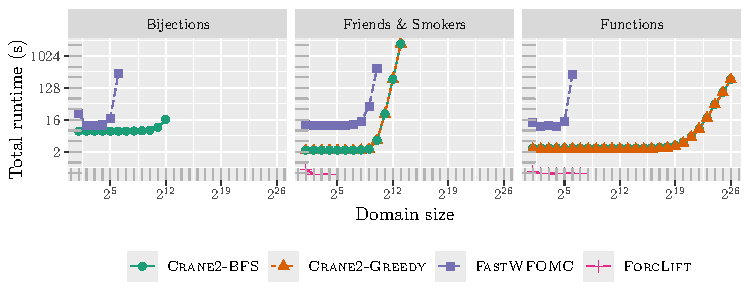
\includegraphics{plot.pdf}
  \caption{The runtime of the algorithms as a function of the domain size. Note
    that both axes are on a logarithmic scale.}\label{fig:plot}
\end{figure*}

\Cref{fig:plot} summarises the experimental results. Only \textsc{FastWFOMC} and
\Cranebfs{} could lift the bijection-counting problem. On this benchmark, the
largest domain sizes that these algorithms could handle were \num{64} and
\num{4096}, respectively. On the other two benchmarks, \textsc{ForcLift} has the
lowest runtime, but, as it is finite-precision, only scales up to domain sizes
of \num{16} and \num{128} in the case of `friends' and `functions',
respectively. Next, \textsc{FastWFOMC} outperforms \textsc{ForcLift} in the case
of `friends' but not `functions': it scales up to domains of size \num{1024} and
\num{64}, respectively. Finally, both \Cranebfs{} and \Cranegreedy{} perform
nearly identically on both of these benchmarks. Similarly to the `bijections'
benchmark, \Cranetwo{} significantly surpasses the other two algorithms, scaling
up to domains of size \num{8192} and \num{67108864}, respectively.

Another aspect of the experimental results worth discussing separately is that
of compilation. As both Julia and Scala use just-in-time (JIT) compilation, both
\textsc{FastWFOMC} and \textsc{ForcLift} take longer when run on the smallest
domain size, as that is when most JIT compilation happens. As \Cranetwo{} is run
only once per benchmark, JIT compilation time is incorporated into its runtime
across all domain sizes. Moreover, while \textsc{ForcLift} compilation is
generally faster than that of \Cranetwo{}, neither is significant in comparison
to inference time. Indeed, typically, \textsc{ForcLift} compilation took around
\SI{0.5}{\second}, while \Cranetwo{} compilation took around \SI{2.3}{\second}.

% 8. Conclusion
% Summary: Briefly summarize the key findings from the experimental results.
% Future Work: Suggest directions for future research based on your findings.

So what do our experiments reveal about which algorithm should one use in
practice? If the formula can be handled by \textsc{ForcLift} and the domain
sizes are reasonably small, it is likely to be the fastest algorithm. In other
cases, \Cranetwo{} is likely to be significantly faster than \textsc{FastWFOMC}
across all domain sizes (but especially with higher domain sizes), assuming the
formula can be handled by both algorithms.

% TODO: run this section through editgpt and grammarly

\section{Conclusion and Future Work}

In this work, we have presented several contributions. First, we have developed
algorithmic techniques to find the base cases of recursive functions generated
by the original \textsc{Crane} algorithm. Second, we have extended the smoothing
procedure of \textsc{ForcLift} and \textsc{Crane} to support base case formulas.
Third, we have proposed an approach to compile function definitions into C++
programs with support for arbitrary-precision arithmetic. Lastly, we have
provided experimental evidence demonstrating that \Cranetwo{} can scale to much
larger domain sizes than \textsc{FastWFOMC} while handling more formulas than
\textsc{ForcLift}.

There are many potential avenues for future work. Specifically, a more thorough
experimental study is needed to understand how WFOMC algorithms compare in terms
of their ability to handle different formulas and their scalability with respect
to domain size. Additionally, further characterisation of the capabilities of
\Cranetwo{} can be explored. For example, \emph{completeness} could be proven
for a fragment of first-order logic such as \Ctwo{} (using a suitable encoding
of counting quantifiers). Moreover, the efficiency of a WFOMC algorithm in
handling a particular formula can be assessed using \emph{fine-grained
  complexity}. In the case of \textsc{Crane} and \Cranetwo{}, this can be done
by analysing the equations~\cite{DBLP:conf/kr/DilkasB23}. By doing so,
efficiency can be reasoned about in a more implementation-independent manner by
making claims about the maximum degree of the polynomial that characterises any
given solution.

\bibliography{paper}

\end{document}
